
\subsubsection{ Region Proposal Network}

The main process followed by most of CNN for Object Detection is:
\begin{enumerate}
\item Fistly, we do feature extraction using as backbone network, the first Convolutional Layers of a known pre-trained CNN such
  as AlexNet, VGG, ResNet etc.
\item Then, we propose regions of interest (ROI) in the image. These regions contain possibly an object, which we are looking for.
\item Finally, we classify each proposed ROI.
\end{enumerate}

From the 3 above steps, the 2nd step is considered to be very important. That is because, in this step, we should choose regions of
the image, which will be classified. Poor choice of ROIs means that the CNN will pass by some object that are located in the image,
because, they were not be proposed to be classified.

\begin{figure}[h]
  \centering
  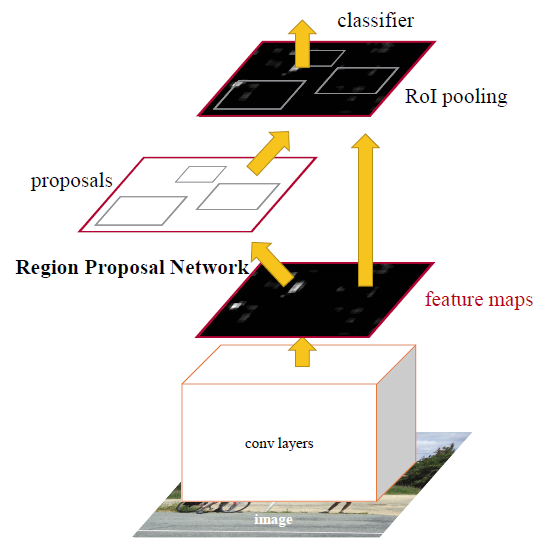
\includegraphics[scale=0.3]{./figures/RPN_structure}
  \caption{ Region Proposal Network's structure}
  \label{fig:rpn_structure}
\end{figure}
The first Object-Detection CNNs use several algorithms for proposing ROIs. For example, R-CNN\cite{DBLP:journals/corr/GirshickDDM13},
and Fast R-CNN\cite{Girshick:2015:FR:2919332.2920125} used Selective Search Algorithm for extracting ROIs.
One of noverlties introduced by the Faster R-CNN\cite{Ren:2015:FRT:2969239.2969250} is \textbf{Region Proposal Network} (RPN). Its
Function is to propose ROIs and its structure can be shown in \ref{fig:rpn_structure}. As we can see, RPN is consisted of:
\begin{itemize}
\item 1 2D Convolutional Layer
\item 1 score layer 
\item 1 regression layer
\end{itemize}

Another basic element of RPN is the \textbf{anchors}. Anchors are predefined boxes used for extracting ROIs. In figure \ref{fig:anchors} is
depicted an exaple of some anchors
\begin{figure}[h]
  \centering
  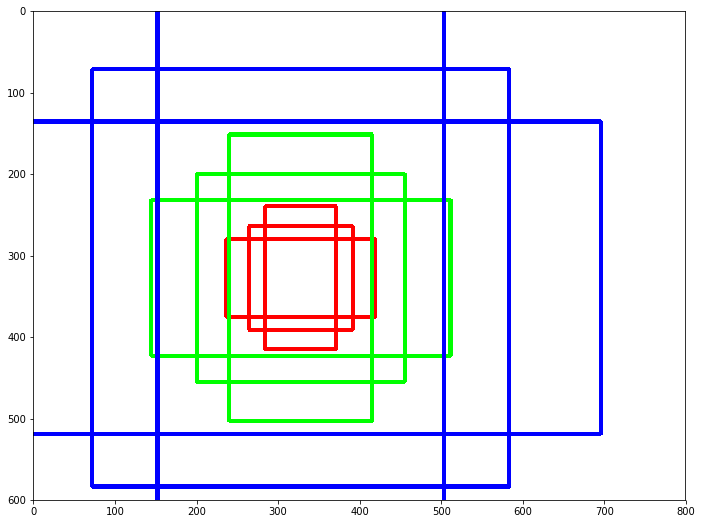
\includegraphics[scale=0.3]{./figures/anchors}
  \caption{ Anchors for pixel (320,320) of an image (600,800) }
  \label{fig:anchors}
\end{figure}

\gr Τα πρώτα \en Object-Detection CNNs \gr χρησιμοποιούν διάφορους αλγόριθμους για να ανακαλύψουν αυτές τις περιοχές. Για παράδειγμα
τα \en R-CNN\cite{DBLP:journals/corr/GirshickDDM13}, Fast R-CNN\cite{Girshick:2015:FR:2919332.2920125} \gr χρησιμοποιούν τον αλγόριθμο
\en Selective Search. \gr Μια από τις καινοτομίες που εισήγαγε το \en Faster R-CNN \gr είναι το \en \textbf{Region Proposal Network} (RPN).
\gr H λειτουργία του είναι να μας προτείνει \en ROIs \gr και την βασική δομή του μπορούμε να την δούμε στην εικόνα \ref{fig:rpn_structure}.
\gr Συνεπώς, το \en RPN \gr αποτελείται από:
\begin{itemize}
\item 1 \en 2D convolutional layer
\item 1 \en layer \gr για \en score
\item 1 \en layer \gr για  \en regression
\end{itemize}

\gr Ένα βασικό στοιχείο του \en RPN \gr είναι τα \en \textbf{anchors}. \gr Τα \en anchors \gr αποτελούν προκαθορισμένα κουτιά που χρησιμοποιεί
το \en RPN \gr προκειμένου να προτείνει \en ROIs. \gr Στην \ref{fig:anchors} μπορούμε να δούμε ένα παράδειγμα κάποιων \en anchors. 
\gr
\begin{figure}[h]
  \centering
  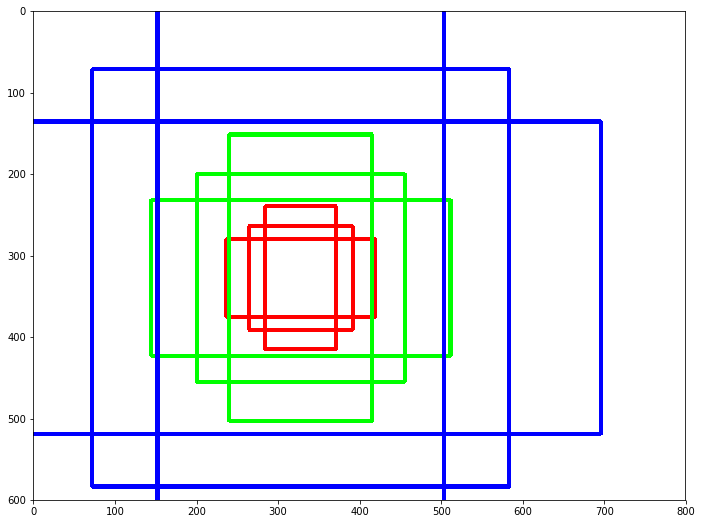
\includegraphics[scale=0.3]{./figures/anchors}
  \caption{\gr Τα \en anchors \gr στο \en pixel (320,320) \gr μιας εικόνας (600,800) }
  \label{fig:anchors}
\end{figure}
\gr Σε κάθε \en pixel \gr των \en feature maps  \gr του \en 2D convolutional layer \gr του \en RPN \gr αντιστοιχούν \en \textbf{k (k=9)} anchors
\gr (3 διαφορετικά \en scales \gr και 3 διαφορετικά \en ratios:  1:1, 1:2, 2:1). \par
\gr To \en RPN \gr λοιπόν, δέχεται ως είσοδο στο \en convolutional layer \gr τα \en feature maps \gr του \en backbone CNN \gr και περνάει την έξοδο του
στο \en scoring layer \gr και στο \en regression layer. 
\gr Tο \en scoring layer \gr παράγει \en 2k scores \gr για κάθε \en pixel \gr του \en feature map. \gr
\gr Αυτά τα \en scores \gr μας λένε πόσο σίγουροι είμαστε για το αν υπάρχει ή όχι κάποιο αντικείμενο στην συγκεκριμένη θέση. Αντίστοιχα, το \en regression
layer \gr παράγει \en 4k \gr μετατοποίσεις, 4 για κάθε ένα \en anchor. \gr Tέλος, κρατάμε ως \en ROIs \gr τα \textit{\en n-\gr πρώτα} \en anchors \gr
με μεγαλύτερο \en score.
